\documentclass[11pt]{beamer}
\usetheme{CambridgeUS}
\usepackage{wrapfig} % bordear la imagen con texto
\usepackage[utf8]{inputenc}
\usepackage{amsmath}
\usepackage{amsfonts}
\usepackage{amssymb}
\usepackage{graphicx}
\usepackage{xcolor}
\author{A.Carolina Ledezma-Carrizalez}
\title{Software Libre en Bioinformática:Abriendo las Puertas a la Ciencia Abierta}
%\setbeamercovered{transparent} 
%\setbeamertemplate{navigation symbols}{} 
%\logo{flisol-venezuela2.png} 
%\institute{} 
%\date{} 
%\subject{} 
\usepackage{Sweave}
\begin{document}
\Sconcordance{concordance:presentacionF25.tex:presentacionF25.Rnw:1 17 1 1 0 321 1}

	\begin{frame}
		\titlepage
		
\includegraphics[width=5cm, height=3cm]{flisol-venezuela2.png}
	\end{frame}
	
%Diapositiva 2 ----------------------------------------------------------------------------------------

	\begin{frame}{Software Libre en Bioinformática: Abriendo las Puertas a la Ciencia Abierta}
	\centering
	\large \textbf {Objetivo: Ofrecer una visión más amplia del papel del software libre en la bioinformática, destacando su importancia para la investigación colaborativa, la transparencia y el avance de la ciencia.}
	\end{frame}
	
%Diapositiva 3	---------------------------------------------------------------------------------------

	\begin{frame}{}
	\centering
	\large \textbf {El software libre es un pilar esencial de la bioinformática moderna y un motor para la ciencia reproducible y colaborativa.}
		\begin{figure}[h!] 
		\centering
		
\includegraphics[width=10cm, height=6cm]{2software-libre.png}
		\end{figure}
	\end{frame}
	
%Diapositiva 4 ----------------------------------------------------------------------------------------
		
	\begin{frame}{Conceptos}
	\centering
	\large \textbf {Ante de comenzar es necesario pensar en estos conceptos:
		\begin{itemize}
		\item Ciencia Abierta
		\item Software Libre
		\item Bioinformática
		\end{itemize}}
	\end{frame}	
	
%Diapositiva 5 ----------------------------------------------------------------------------------------	

	\setbeamercolor{background canvas}{bg=lightgray!40}	
	\begin{frame}{Conceptos - Ciencia Abierta - Venezuela}
	\centering
En las Recomendación de la UNESCO (sept.2023)
"La ciencia abierta es un conjunto de principios y prácticas que tienen como objetivo hacer que la investigación científica desde todos sea accesible a todos para los beneficios de los científicos y de la sociedad en su conjunto. La ciencia abierta consiste en asegurarse no sólo de que el conocimiento científico sea accesible, sino también de que la producción de ese conocimiento en sí sea inclusiva, equitativa y sostenible."
	\end{frame}
	
%Diapositiva 6 ----------------------------------------------------------------------------------------

	\begin{frame}{Conceptos - Ciencia Abierta - Venezuela}
	\centering
"La Ciencia Abierta se define como un constructo inclusivo que combina diversos movimientos y prácticas con el fin de que los conocimientos científicos multilingües estén abiertamente disponibles y sean accesibles para todos, así como reutilizables por todos, se incrementen las colaboraciones científicas y el intercambio de información en beneficio de la ciencia y la sociedad, y se abran los procesos de creación, evaluación y comunicación de los conocimientos científicos a los agentes sociales más allá de la comunidad científica tradicional."
	\end{frame}	
	
%Diapositiva 7 ----------------------------------------------------------------------------------------

	\begin{frame}{Logros, Iniciativas y Referentes - Ciencia Abierta - Venezuela}
	\begin{columns} % Inicia el entorno de columnas
        		% Le asignamos un ancho (ej: 50% del ancho del texto de la diapositiva)
			\begin{column}{0.5\textwidth}
				\begin{itemize}
				\item Identificación y sistematización de los principales y referentes de CA en el país.
				\item Libro “Ciencia Abierta en Venezuela”
				\item Alianza Científico Campesina 
				\item Fundación INFOCENTRO
				\item Sistema Nacional de Orquesta Juveniles e Infantiles de Venezuela.
				\end{itemize}           		
        		\end{column}
        		% Le asignamos el ancho restante (ej: 50% del ancho del texto de la diapositiva)
        		\begin{column}{0.5\textwidth}
            % Colocamos la imagen dentro de un entorno figure 
            		\begin{itemize}
            		\item Las comunidades de software libre.
            		\item Comunalización de la Ciencia
            		\end{itemize}
            		\textbf{recientes experiencias de CA:}
            		\begin{itemize}
            		\item Universidad Nacional de las Ciencias "Humberto Fernández Moran" teniendo base la CA (postulaciones)
            		\item CEBISA Centro de Formación en Biotecnología de Semillas
            		\end{itemize}
        		\end{column}
    		\end{columns} % Finaliza el entorno de columnas
    		\footnote{Dra. Caroly Higuera N. punto focal de Ciencia abierta de Venezuela -UNESCO} 
	\end{frame}
	
%Diapositiva 8 ----------------------------------------------------------------------------------------

	\setbeamercolor{background canvas}{bg=white}
	\begin{frame}{Conceptos - Software Libre}

  		El Software Libre y de Código Abierto (SLCA), FOSS (Free and Open Source Software) o FLOSS (Free/Libre Open Source Software)- código fuente está accesible.
 	
	\end{frame}
	
%Diapositiva 9 ----------------------------------------------------------------------------------------

	\begin{frame}{¿Qué es el Software Libre? y ¿Por Qué Importa?}

		\textbf{Las 4 Libertades esenciales} 
		
		\begin{itemize}
		\item \textbf{La Libertad 0:} La libertad de ejecutar el programa como se desee, con cualquier propósito.
		\item \textbf{La Libertad 1:} La libertad de estudiar cómo funciona el programa y modificarlo para que haga lo que deseas.
		\item \textbf{La Libertad 2:} La libertad de redistribuir copias para poder ayudar a tu vecino.
		\item \textbf{La Libertad 3:} La libertad de distribuir copias de tus versiones modificadas a terceros.
		\end{itemize}
	\end{frame}
	
%Diapositiva 10 ----------------------------------------------------------------------------------------
	
	\begin{frame}{FOSS Free and Open Source Software ¿Por qué FOSS en Bioinformática?}	
 Énfasis en la libertad, no solo el costo cero.
        \begin{itemize}        
		\item Accesibilidad: Elimina barreras económicas para investigadores, estudiantes e instituciones (especialmente en países en desarrollo).
		\item Transparencia y Reproducibilidad: ¡Crucial para la ciencia! El código abierto permite verificar algoritmos, entender métodos y replicar resultados.
		\item Colaboración: Fomenta el desarrollo comunitario, la revisión por pares del código y la construcción sobre trabajos previos.
		\item Personalización: Permite adaptar herramientas a necesidades específicas de investigación.
		\item Innovación: Acelera el desarrollo de nuevos métodos y algoritmos.
		\end{itemize}
	\end{frame}
	
%Diapositiva 11 ----------------------------------------------------------------------------------------
	
	\begin{frame}{Canaima}	
	
	https://canaima.softwarelibre.gob.ve/
	
	\begin{figure}[h!] 
    				\centering
				\includegraphics[width=6cm, height=4cm]{Canaima.png}
			\end{figure}	
	\end{frame}

%Diapositiva 12 ----------------------------------------------------------------------------------------

	\begin{frame}{El software libre es un habilitador clave de la Ciencia Abierta}
		\textbf {Valores de Ciencia Abierta}
 		\begin{itemize}
			\item Calidad e integridad
			\item Benefectivo colectivo
			\item Equidad y equidad
			\item Diversidad e inclusión
 		\end{itemize}	
		\textbf {Principios rectores}
 		 \begin{itemize}
			\item Transparencia, escrutinio, crítica y reproducibilidad
			\item Igualdad de oportunidades
			\item Responsabilidad, respeto y rendición de cuentas
			\item Colaboración, participación e inclusión
			\item Flexibilidad
			\item Sostenibilidad
 		\end{itemize}
	\end{frame}	
	
%Diapositiva 13 ----------------------------------------------------------------------------------------

	\begin{frame}{Conceptos - Bioinformática}
		\textit{Intersección entre biología, ciencias de la computación, matemáticas y estadística para analizar e interpretar datos biológicos.}
			\begin{figure}[h!] 
    				\centering
				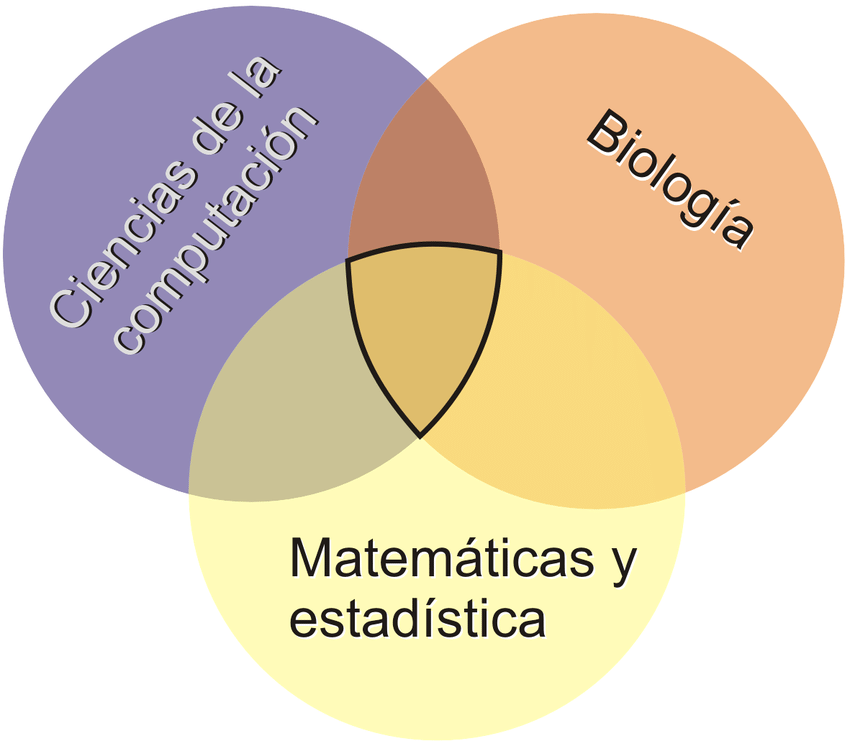
\includegraphics[width=6cm, height=4cm]{interaccion-de-tres-ciencias-basicas.png}
			\end{figure}
	\end{frame}
	
%Diapositiva 14 ------------------------------------------------------------------------------------------

	\begin{frame}{Explosion de Datos}
La tecnología abarató la secuenciación y generó una avalancha de datos ómicos. Pero fue el software libre el que nos dio las herramientas gratis y abiertas para poder analizar toda esa información.

Sin ese software, solo unos pocos hubieran podido estudiar los datos, y el avance científico habría sido mucho más lento y cerrado. La explosión de datos y el software libre van totalmente de la mano.
El Papel del Software: Es la lente a través de la cual vemos y entendemos los datos biológicos complejos.
	\end{frame}
	
%Diapositiva 15 ------------------------------------------------------------------------------------------	

	\begin{frame}{Datos Ómicos- Las Ómicas }
		\begin{wrapfigure}{r}{0.55 \textwidth} % l: izquierda, 0.3\textwidth: ancho 30% del ancho del texto
    		\centering % Opcional: centra la imagen dentro del espacio asignado
    		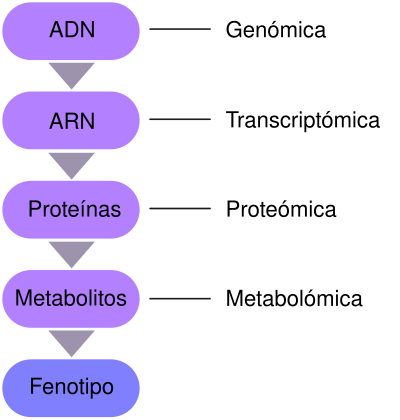
\includegraphics[width=0.7\linewidth]{Omics.png} % Ajusta la imagen al ancho del wrapfigure
    		\caption{Multiómica.} % Opcional: pie de figura
    		\label{fig:Multiómica} % Opcional: etiqueta para referenciar
		\end{wrapfigure}
Es un grupo de disciplinas 
en biología como ...

Estas disciplinas tienen como objetivo la identificación, caracterización y cuantificación de conjuntos de biomoléculas y procesos moleculares que originan la estructura, función y dinámicas de células, tejidos y organismos
	\end{frame}

%Diapositiva 16 -------------------------------------------------------------------------------------------

	\begin{frame}{El Ecosistema FOSS en Bioinformática - Un Vistazo General}

Diversidad de Herramientas: Cubren todo el espectro del análisis bioinformático.
Categorías Principales :
		 \begin{itemize}
			\item Análisis de Secuencias (BLAST, Bowtie, STAR)
			\item Ensamblaje de Genomas (SPAdes, Canu)
			\item Análisis Filogenético (PhyML, RAxML)
			\item Análisis Estructural (PyMOL - versión libre disponible, VMD)
			\item Estadística y Visualización (¡Aquí entra R!)
			\item Gestión de Flujos de Trabajo (Nextflow, Snakemake)
 		\end{itemize}
	\end{frame}
	
%Diapositiva 17 ------------------------------------------------------------------------------------------	

	\begin{frame}{R - El Corazón Estadístico y Gráfico de la Bioinformática}
		\begin{wrapfigure}[13]{l}{0.55 \textwidth} % l: izquierda, 0.3\textwidth: ancho 30% del ancho del texto
    		\centering % Opcional: centra la imagen dentro del espacio asignado
    		
\includegraphics[width=1 \linewidth]{R31.png} % Ajusta la imagen al ancho del wrapfigure
    		\caption{Logo R} % Opcional: pie de figura
    		\label{fig:R} % Opcional: etiqueta para referenciar
		\end{wrapfigure}
¿Qué es R? Lenguaje y entorno para computación estadística y gráficos.
Es una herramienta fundamental en el mundo de la ciencia de datos, la estadística, la investigación académica y la industria para el análisis, la manipulación, la visualización y el reporte de datos. Es potente, flexible y, al ser de código abierto, accesible para todos.
Es software libre y de código abierto.
	\end{frame}
	
%Diapositiva 18 ------------------------------------------------------------------------------------------

	\begin{frame}   
    % \frametitle{}
    		\begin{columns} % Inicia el entorno de columnas
        		% Le asignamos un ancho (ej: 50% del ancho del texto de la diapositiva)
			\begin{column}{0.5\textwidth}
            		\textbf{Capacidades Gráficas:} Potentes librerías como ggplot2 para visualizaciones de alta calidad.
            		\textbf{Comunidad Enorme:} Gran soporte, tutoriales, foros. 
           		https://github.com/z3tt
        		\end{column}
        		% Le asignamos el ancho restante (ej: 50% del ancho del texto de la diapositiva)
        		\begin{column}{0.5\textwidth}
            % Colocamos la imagen dentro de un entorno figure 
            		\begin{figure}
            		    % Centrar la imagen dentro de su columna
                		\centering
                		% Incluye la imagen. Usa \linewidth para que la imagen se ajuste al ancho de la columna
                		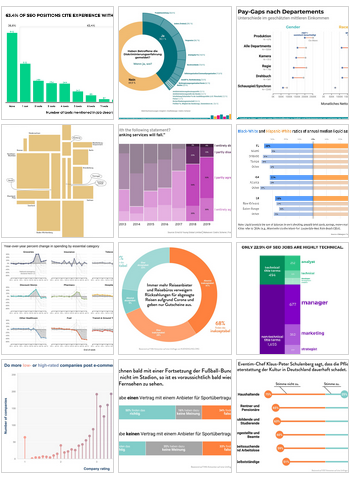
\includegraphics[width= 0.9 \linewidth]{cedri2.png}
                		\caption{Cédric Scherer} % Pie de figura
                		\label{fig:cedric_scherer} % Etiqueta si necesitas referenciarla
            		\end{figure}
        		\end{column}
    		\end{columns} % Finaliza el entorno de columnas
	\end{frame}
	
%Diapositiva 19 ---------------------------------------------------------------------------------------
	
	\begin{frame}
		\begin{wrapfigure}{l}{0.7 \textwidth} % l: izquierda, 0.3\textwidth: ancho 30% del ancho del texto
	    		\centering % Opcional: centra la imagen dentro del espacio asignado
  	  		\includegraphics[width=1\linewidth]{AllisonHorst.png} 
   	 		\caption{Allison Horst https://github.com/allisonhorst} 
    			\label{fig:Allison Horst} % Opcional: etiqueta para referenciar
		\end{wrapfigure}
			\textbf {Reproducibilidad:} 
Facilita la creación de informes y análisis reproducibles (R Markdown, Quarto).
	\end{frame}
	
%Diapositiva 20 ---------------------------------------------------------------------------------------

	\begin{frame}
		\centering
		\LARGE \textbf {¿Por qué es tan dominante en Bioinformática?}
	\end{frame}
	
%Diapositiva 21 ---------------------------------------------------------------------------------------

	\begin{frame}{Bioconductor- R} 
		\begin{wrapfigure}{r}{0.55 \textwidth} % l: izquierda, 0.3\textwidth: ancho 30% del ancho del texto
    		\centering % Opcional: centra la imagen dentro del espacio asignado
    		
\includegraphics[width=0.8\linewidth]{bioconductor.png} % Ajusta la imagen al ancho del wrapfigure
    		\caption{Logo Bioconductor.} % Opcional: pie de figura
    		\label{fig:Bioconductor} % Opcional: etiqueta para referenciar
	\end{wrapfigure}
 ¡La clave! Es un proyecto de código abierto (open source) y desarrollo abierto que se dedica a crear y compartir herramientas de software para el análisis de datos biológicos de alto rendimiento, especialmente en áreas como la genómica y la biología molecular.

Está basado principalmente en R.Ejemplos de paquetes Bioconductor: DESeq2/edgeR (expresión diferencial), limma, GenomicRanges.
	\end{frame}
	
%Diapositiva 22 ---------------------------------------------------------------------------------------

	\begin{frame}{Más Allá de R - Otras Herramientas FOSS Imprescindibles}

 		\begin{itemize}
 			\item Python:Otro gigante en bioinformática. Librerias de Python
					\begin{itemize}
					\item Biopython (manipulación de secuencias y formatos)
					\item NumPy/SciPy(cálculo científico)
					\item Pandas (manipulación de datos)
					\item Matplotlib Seaborn(visualización)
					\item Scikit-learn (Machine Learning)
					\end{itemize}
			\item Herramientas de Línea de Comandos (CLI):Fundamentales para procesar grandes volúmenes de datos y automatizar tareas.
 			
					\begin{itemize}
					\item SAMtools / BCFtools: Manipulación de alineamientos y variantes genéticas. Indispensables.
					\item BEDTools: Herramientas para trabajar con intervalos genómicos.
					\end{itemize}
		\end{itemize}	
 	\end{frame}
 	
%Diapositiva 23 ----------------------------------------------------------------------------------------

	\begin{frame}
 		\begin{itemize}	
			\item BLAST (NCBI National Center for Biotechnology Information): Aunque no es FOSS en el sentido estricto de licencia para modificar todo, la herramienta es libremente utilizable y distribuible, y es un estándar de facto.
			\item GATK Genome Analysis Toolkit(parcialmente):Históricamente complejo en licencias, pero partes clave y versiones anteriores son accesibles y ampliamente usadas.
			\item Gestores de Flujos de Trabajo (Workflows):Nextflow / Snakemake: Esenciales para crear pipelines de análisis complejos, reproducibles y escalables. Utilizan herramientas FOSS subyacentes.
 		\end{itemize}
	\end{frame}
	
%Diapositiva 24 ----------------------------------------------------------------------------------------	

	\begin{frame}
	\centering
	\large \textbf{por favor recuerda que vale la pena ser libre, aunque es comodo pulsar next}
	\begin{figure}[h!] 
		\centering
		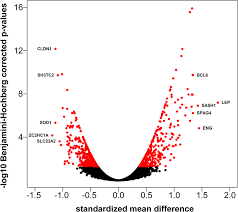
\includegraphics[width=5cm, height=3cm]{volcan.png}
		\end{figure}
	
	¡Muchas gracias por su atencion!
	\end{frame}
\end{document}
